% Copyright 2016 by Wang Kunzhen <wangkunzhen1993@gmail.com>.
%
% This is a latex template adapted from Till Tantau's Beamer template.
% It adds theme customizations for the convenience of users from the
% National University of Singapore. 
% 
% In principle, this file can be redistributed and/or modified under
% the terms of the GNU Public License, version 2.
%
% However, this file is supposed to be a template to be modified
% for your own needs. For this reason, if you use this file as a
% template and not specifically distribute it as part of a another
% package/program, I grant the extra permission to freely copy and
% modify this file as you see fit and even to delete this copyright
% notice. 

\documentclass[xcolor=dvipsnames]{beamer}

% There are many different themes available for Beamer. A comprehensive
% list with examples is given here:
% http://deic.uab.es/~iblanes/beamer_gallery/index_by_theme.html
% You can uncomment the themes below if you would like to use a different
% one:
%\usetheme{AnnArbor}
%\usetheme{Antibes}
%\usetheme{Bergen}
% \usetheme{Berkeley}
%\usetheme{Berlin}
%\usetheme{Boadilla}
% \usetheme{boxes}
%\usetheme{CambridgeUS}
%\usetheme{Copenhagen}
%\usetheme{Darmstadt}
%\usetheme{default}
\usetheme{Frankfurt}
%\usetheme{Goettingen}
%\usetheme{Hannover}
% \usetheme{Ilmenau}
% \usetheme{JuanLesPins}
% \usetheme{Luebeck}
% \usetheme{Madrid}
% \usetheme{Malmoe}
%\usetheme{Marburg}
% \usetheme{Montpellier}
% \usetheme{PaloAlto}
% \usetheme{Pittsburgh}
% \usetheme{Rochester}
% \usetheme{Singapore}
% \usetheme{Szeged}
% \usetheme{Warsaw}

\definecolor{nus-orange}{RGB}{239,124,0} 
\definecolor{nus-white}{RGB}{255,255,255}
\definecolor{nus-blue}{RGB}{0,61,124}
\definecolor{nus-black}{RGB}{0,0,0}

% Uncomment this section if you want the title background for each slide to be gradient like decaying from nus-orange to nus-white.
% \useoutertheme{shadow}
% \usepackage{tikz}
% \usetikzlibrary{shadings}
% \colorlet{titleleft}{nus-orange}
% \colorlet{titleright}{nus-orange!45!nus-white}
% \makeatletter
% \pgfdeclarehorizontalshading[titleleft,titleright]{beamer@frametitleshade}{\paperheight}{%
%   color(0pt)=(titleleft);
%   color(\paperwidth)=(titleright)}
% \makeatother
% End of gradient slide title effect.

\setbeamercolor{section in head/foot}{bg=nus-blue, fg=nus-white}
\setbeamercolor{subsection in head/foot}{bg=nus-blue, fg=nus-white}
\setbeamercolor{frametitle}{bg=nus-orange, fg=nus-white}
\setbeamercolor{title}{bg=nus-orange, fg=nus-white}
\setbeamercolor{alerted text}{fg=nus-orange}
\setbeamercolor{block title}{fg=nus-white}
\setbeamercolor{block body}{fg=nus-black}

\setbeamertemplate{theorems}[numbered]
\setbeamertemplate{propositions}[numbered]

\setbeamertemplate{bibliography item}{\insertbiblabel}

\setbeamertemplate{title page}[default][colsep=-4bp,rounded=true, shadow=true]

\usefonttheme[onlymath]{serif}
\setbeamertemplate{footline}[totalframenumber]

\addtobeamertemplate{navigation symbols}{}{
  \hspace{1em} \raisebox{1.35pt}{\usebeamerfont{footline}%
\insertframenumber/\inserttotalframenumber} }

\renewcommand\qedsymbol{$\blacksquare$}
% \setbeamertemplate{qed symbol}{$\blacksquare$}

\usepackage{braket}
\usepackage{multirow}
\usepackage{adjustbox} % allow tables to take up the space they need
\usepackage{graphicx} % allows figures to be inserted and scaled
\usepackage{listings} % allows for source code blocks
\usepackage{fancyvrb} % robust verbatim
\usepackage{siunitx} % allows SI units to be formatted

\usepackage[backend=biber, style=ieee]{biblatex}  
\addbibresource{../wiring.bib}
% \usepackage{hyperref} % hyperlinks
% \hypersetup{%
%   colorlinks=true,
%   linkcolor=purple,
%   urlcolor=blue
% }
\graphicspath{ {../images/} }

\newcommand{\concat}{\mathbin{\Vert}} % string concatenation operator
\newcommand{\rep}{\stackrel{r}{=}} % enable stacked r and = for representation
\newcommand{\?}{\mathrel{?}} % ternary operator

\DeclareMathOperator*{\argmin}{argmin}
\DeclareMathOperator*{\argmax}{argmax}
\newcommand{\norm}[1]{\left\lVert#1\right\rVert} % define norm
\newcommand{\abs}[1]{\left\lvert#1\right\rvert} % define abs
\newcommand{\Dif}{\mathop{}\!\mathrm{D}} % Difference operator
\newcommand{\dif}{\mathop{}\!\mathrm{d}} % differential d
\newcommand{\ceil}[1]{\left\lceil#1\right\rceil} % enables \ceil{} for ceil delimiter
\newcommand{\floor}[1]{\left\lfloor#1\right\rfloor} % enables \floor{} for floor delimiter
\newcommand{\cvec}[1]{\boldsymbol{\mathbf{#1}}}    % shortcut for column vectors
\newcommand{\rvec}[1]{\boldsymbol{\mathbf{#1}}^{T}} % shortcut for transposed row vectors
\newcommand{\Z}{\mathbb{Z}} % for integers
\newcommand{\R}{\mathbb{R}} % for reals
\newcommand{\C}{\mathbb{C}} % for complex
\newcommand{\dintv}[2]{\left\{#1,\ldots,#2\right\}}
\newcommand{\ocintv}[2]{\left(#1,#2\right]}
\newcommand{\cointv}[2]{\left[#1,#2\right)}
\newcommand{\ccintv}[2]{\left[#1,#2\right]}
\newcommand{\oointv}[2]{\left(#1,#2\right)}
\newcommand{\matr}[1]{\left[\mathbf{#1}\right]} % shortcut for matrices
\newcommand{\matrp}[2]{\left[\mathbf{#1}#2\right]} % shortcut for matrices with subscripts/superscripts
\newcommand{\rv}[1]{\boldsymbol{\mathbf{#1}}} % random variable
\newcommand{\Tr}{\mathrm{Tr}} % enables trace operator
\newcommand{\id}{\mathrm{id}} % enables id operator
\newcommand{\E}{\mathbb{E}} % expectation
\newcommand{\angleb}[1]{\left\langle #1 \right\rangle} % physicist's notation for mean
\newcommand{\Var}{\mathrm{Var}} % variance

\newenvironment{Tabular}[1] % less cramped tables
{\def\arraystretch{1.75}\begin{tabular}{#1}}
{\end{tabular}}
\newenvironment{Array*}[1] % less cramped display mode arrays
{\def\arraystretch{1.75}\everymath={\displaystyle}\[\begin{array}{#1}}
{\end{array}\]}
\newenvironment{Array}[1] % less cramped display mode arrays
{\def\arraystretch{1.75}\everymath={\displaystyle}\begin{equation}\begin{array}{#1}}
{\end{array}\end{equation}}
\newenvironment{displaytable}[1] % environment for a simple inline table to present some information
{\vspace\abovedisplayskip\begin{center}\begin{tabular}{#1}}
{\end{tabular}\end{center}\vspace\belowdisplayskip}

\usepackage{mathtools}
\usepackage{tikz}
\usepackage{tikzscale} % include .tikz files with includegraphics and scale them
\usetikzlibrary{shapes, shapes.geometric, automata, positioning, arrows.meta, decorations.markings,decorations.pathreplacing, intersections, math, 3d, backgrounds}
\newcommand{\expandidx}[2]{%
  \expandafter#1\expandafter{\the\numexpr#2\relax}%
}

\tikzset{%
  >={Stealth}, % makes the arrow heads bold
  node distance=3cm, % specifies the minimum distance between two nodes. Change if necessary.
  every state/.style={thick, fill=gray!10}, % sets the properties for each ’state’ node
  initial text=$ $, % sets the text that appears on the start arrow
  % style to apply some styles to each segment of a path
  on each segment/.style={
    decorate,
    decoration={
      show path construction,
      moveto code={},
      lineto code={
        \path [#1]
        (\tikzinputsegmentfirst) -- (\tikzinputsegmentlast);
      },
      curveto code={
        \path [#1] (\tikzinputsegmentfirst)
        .. controls
        (\tikzinputsegmentsupporta) and (\tikzinputsegmentsupportb)
        ..
        (\tikzinputsegmentlast);
      },
      closepath code={
        \path [#1]
        (\tikzinputsegmentfirst) -- (\tikzinputsegmentlast);
      },
    },
  },
  % style to add an arrow in the middle of a path
  mid arrow/.style={postaction={decorate,decoration={
        markings,
        mark=at position .5 with {\arrow[#1]{stealth}}
  }}},
}


\tikzset{%
  % simple black circle at node
  point/.style={circle,draw,inner sep=0pt,minimum size=3pt,fill=black},
  % coin with label and colours
  % TODO DOES NOT WORK
  set coin/.code={\pgfqkeys{/tikz/coin}{#1}},
  set coin={bg/.initial=black, fg/.initial=white},
  coin/.style={
    set coin={#1},
    postaction={
      circle,draw=\pgfkeysvalueof{/tikz/coin/fg},
      text=\pgfkeysvalueof{/tikz/coin/fg},
      fill=\pgfkeysvalueof{/tikz/coin/bg}
    }
  }
}

\RequirePackage{luatex85}
% Default preamble
\usepackage{pgfplots}
\pgfplotsset{compat=newest}
\usepgfplotslibrary{groupplots}
\usepgfplotslibrary{polar}
\usepgfplotslibrary{smithchart}
\usepgfplotslibrary{statistics}
\usepgfplotslibrary{dateplot}
\usepgfplotslibrary{ternary}
\usetikzlibrary{arrows.meta}
\usetikzlibrary{backgrounds}
\usepgfplotslibrary{patchplots}
\usepgfplotslibrary{fillbetween}
\pgfplotsset{%
  layers/standard/.define layer set={%
    background,axis background,axis grid,axis ticks,axis lines,axis tick labels,pre main,main,axis descriptions,axis foreground%
    }{grid style= {/pgfplots/on layer=axis grid},%
    tick style= {/pgfplots/on layer=axis ticks},%
    axis line style= {/pgfplots/on layer=axis lines},%
    label style= {/pgfplots/on layer=axis descriptions},%
    legend style= {/pgfplots/on layer=axis descriptions},%
    title style= {/pgfplots/on layer=axis descriptions},%
    colorbar style= {/pgfplots/on layer=axis descriptions},%
    ticklabel style= {/pgfplots/on layer=axis tick labels},%
    axis background@ style={/pgfplots/on layer=axis background},%
    3d box foreground style={/pgfplots/on layer=axis foreground},%
  },
}

\newcommand{\frI}{\mathfrak{I}}
\newcommand{\frX}{\mathfrak{X}}
\newcommand{\rvX}{\rv{X}}
\newcommand{\frA}{\mathfrak{A}}
\newcommand{\frC}{\mathfrak{C}}
\newcommand{\frR}{\mathfrak{R}}
\newcommand{\Dist}{\mathcal{D}}
\newcommand{\DistRI}{\Dist(\frR, \frI)}
\newcommand{\Fail}{\mathcal{F}}
\newcommand{\IdealObsv}{\mathcal{I}}

\newcommand{\psubs}{p_{\rm subs}}
\newcommand{\pimpr}{p_{\rm impr}}

\newcommand{\sM}{\mathcal{M}}
\newcommand{\sN}{\mathcal{N}}
\newcommand{\sS}{\mathcal{S}}
\newcommand{\sK}{\mathcal{K}}
\newcommand{\sT}{\mathcal{T}}
\newcommand{\sH}{\mathcal{H}}
\newcommand{\sV}{\mathcal{V}}
\newcommand{\sW}{\mathcal{W}}
\newcommand{\sX}{\mathcal{X}}
\newcommand{\sY}{\mathcal{Y}}
\newcommand{\sZ}{\mathcal{Z}}
\newcommand{\cE}{\mathcal{E}}
\newcommand{\cF}{\mathcal{F}}
\newcommand{\cP}{\mathcal{P}}

\newcommand{\AU}{\mathrm{AU}_{2}}
\newcommand{\AXU}{\mathrm{AXU}_{2}}
\newcommand{\ASU}{\mathrm{ASU}_{2}}
\newcommand{\eAU}{\epsilon\text{-}\AU}
\newcommand{\eAXU}{\epsilon\text{-}\AXU}
\newcommand{\eASU}{\epsilon\text{-}\ASU}

\newcommand{\meas}{\rm meas}
\newcommand{\perm}{\rm perm}
\newcommand{\pe}{\rm pe}
\newcommand{\pa}{\rm pa}
\newcommand{\ir}{\rm ir}
\newcommand{\leakir}{\mathrm{leak}_{\ir}}
\newcommand{\auth}{\rm auth}
\newcommand{\key}{\rm key}
\newcommand{\rob}{\rm rob}
\newcommand{\cor}{\rm cor}
\newcommand{\secur}{\rm sec}
\newcommand{\erob}[1]{\epsilon_{\rob}^{(#1)}}

\newcommand{\HC}{\mathrm{HC}}
\newcommand{\MC}{\mathrm{MC}}

\newcommand{\Ls}{\mathcal{L}}
\newcommand{\Qs}{\mathcal{Q}}
\newcommand{\NSs}{\mathcal{NS}}
\newcommand{\PR}{\mathrm{PR}}
\newcommand{\sWB}{\mathcal{WB}}
\newcommand{\sk}{\rm sk}
\newcommand{\DW}{\rm DW}
\newcommand{\std}{\rm std}
\newcommand{\crit}{\rm crit}

\setbeameroption{hide notes} % Only slides
% \setbeameroption{show only notes} % Only notes
% \setbeameroption{show notes on second screen=right} % Both
\setbeamertemplate{note page}[plain]

\title{Device-independent quantum key distribution with local wiring}

\author{John Khoo}

\institute[National University of Singapore]
{
  Department of Electrical and Computer Engineering \\ \& Department of Computer Science \\
  National University of Singapore
}

\titlegraphic{
  
\includegraphics[width=2cm]{nus-logo}
}

\date{\today}

% Uncomment this, if you want the table of contents to pop up at
% the beginning of each subsection:
\AtBeginSubsection[]
{
  \begin{frame}<beamer>{Outline}
    \tableofcontents[currentsection,currentsubsection]
  \end{frame}
}

\begin{document}

\begin{frame}
  \titlepage
\end{frame}

\begin{frame}{Outline}
  \tableofcontents
\end{frame}

\section*{Introduction}
\begin{frame}{Quantum Key Distribution (QKD)}
  \begin{itemize}[<+->]
    \item Quantum processes are \alert{fundamentally indeterministic}
    \item This can be used for \alert{cryptographic purposes}
    \item Quantum correlations can be \alert{guaranteed to be private}
    \item We can \alert{distill secret keys} from them
  \end{itemize}
\end{frame}

\note{
  Like good engineers, the first thing we try to do is figure out how we can use this.
}

\begin{frame}{Device-Independent Quantum Key Distribution (DIQKD)}
  \begin{itemize}[<+->]
    \item Many \alert{assumptions} about devices needed for QKD security
    \item Impossible to rule out \alert{all possible device flaws}
    \item DIQKD:\ certify privacy using \alert{device statistics} from \alert{Bell tests}
  \end{itemize}
\end{frame}

\note{
  While our protocols may be secure in theory, the devices we choose to implement them may violate the assumptions of our proofs.

  The behaviour is fully parametrised by a small set of easily measurable variables.
}

\begin{frame}{Wiring}
  \begin{itemize}[<+->]
    \item Connect multiple boxes together with wires
    \item Overall system \alert{can still be used for DIQKD}
    \item Will have different statistics
    \item \alert{Can this be helpful for DIQKD?}
  \end{itemize}
\end{frame}

\begin{frame}{Objective}
  \begin{itemize}[<+->]
    \item The dream: \alert{efficient algorithm} to find \alert{best wiring}
    \item If not possible, \alert{find out why}
    \item Interim presentation: review approaches and techniques tried
  \end{itemize}
\end{frame}

\section{Preliminaries}

\subsection{Review}

\begin{frame}{Bell Tests}
  \begin{onlyenv}<1>
    \begin{figure}
      \centering
      \begin{tikzpicture}
        \tikzmath{\rows = 5; \cols = 3; \intra = 2; \inter = 2; \rheight = 1;
        \nrowv = \rheight+\rheight; \theight = \rows*\rheight; 
        \colm = \cols-1; \ncolh = \inter+\intra; \twidth = \colm*\inter+\cols*\intra;}
        \draw (0,0) node {Alice} ++(\intra,0) node {Bob} ++(\inter,0) node {Alice} ++(\intra,0) node {Bob} ++(\inter,0) node {Alice} ++(\intra,0) node {Bob};
        \foreach \v in {\rheight,\nrowv,...,\theight} {
          \foreach \h in {0,\ncolh,...,\twidth} {
            \tikzmath{int \a, \b, \x, \y;
              \a = random(0,1); \b = random(0,1); \x = random(0,1); \y = random(0,1);
              if \a == 1 then { let \aval = H; } else { let \aval = T; };
              if \b == 1 then { let \bval = H; } else { let \bval = T; };
              if \x == 1 then { let \afg = black; let \abg = white; } else { let \afg = white; let \abg = black; };
              if \y == 1 then { let \bfg = black; let \bbg = white; } else { let \bfg = white; let \bbg = black; };
            }

            % TODO DOES NOT WORK
            % \draw (\h, \v) node[coin={bg = \abg, fg = \afg}] {\aval} ++(\intra,0) node[coin={bg = \bbg, fg = \bfg}] {\bval};
            \draw (\h, \v) node[circle,draw=\afg, text=\afg, fill=\abg,] {\aval} ++(\intra,0) node[circle,draw=\bfg, text=\bfg, fill=\bbg, ] {\bval}; 
          }
        }

        \tikzmath{\ilineh = \intra+0.5*\inter; \nlineh = \ilineh+\intra+\inter;}
        \foreach \h in {\ilineh, \nlineh} {
          \path[draw=black] (\h, -0.5*\rheight) -- (\h, \theight+0.5*\rheight);
        }
      \end{tikzpicture}
      \caption{Uncorrelated statistics}%
    \end{figure}
  \end{onlyenv}

  \begin{onlyenv}<2>
    \begin{figure}
      \centering
      \begin{tikzpicture}
        \tikzmath{\rows = 5; \cols = 3; \intra = 2; \inter = 2; \rheight = 1;
        \nrowv = \rheight+\rheight; \theight = \rows*\rheight; 
        \colm = \cols-1; \ncolh = \inter+\intra; \twidth = \colm*\inter+\cols*\intra;}
        \draw (0,0) node {Alice} ++(\intra,0) node {Bob} ++(\inter,0) node {Alice} ++(\intra,0) node {Bob} ++(\inter,0) node {Alice} ++(\intra,0) node {Bob};
        \foreach \v in {\rheight,\nrowv,...,\theight} {
          \foreach \h in {0,\ncolh,...,\twidth} {
            \tikzmath{int \a, \b, \x, \y;
              \x = random(0,1); \y = random(0,1);
              if \x == 1 then { let \afg = black; let \abg = white; } else { let \afg = white; let \abg = black; };
              if \y == 1 then { let \bfg = black; let \bbg = white; } else { let \bfg = white; let \bbg = black; };
            }

            \draw (\h, \v) node[circle,draw=\afg, text=\afg, fill=\abg,] {H} ++(\intra,0) node[circle,draw=\bfg, text=\bfg, fill=\bbg, ] {H}; 
          }
        }

        \tikzmath{\ilineh = \intra+0.5*\inter; \nlineh = \ilineh+\intra+\inter;}
        \foreach \h in {\ilineh, \nlineh} {
          \path[draw=black] (\h, -0.5*\rheight) -- (\h, \theight+0.5*\rheight);
        }
      \end{tikzpicture}
      \caption{Locally correlated statistics}%
    \end{figure}
  \end{onlyenv}

  \begin{onlyenv}<3>
    \begin{figure}
      \centering
      \begin{tikzpicture}
        \tikzmath{\rows = 5; \cols = 3; \intra = 2; \inter = 2; \rheight = 1;
        \nrowv = \rheight+\rheight; \theight = \rows*\rheight; 
        \colm = \cols-1; \ncolh = \inter+\intra; \twidth = \colm*\inter+\cols*\intra;}
        \draw (0,0) node {Alice} ++(\intra,0) node {Bob} ++(\inter,0) node {Alice} ++(\intra,0) node {Bob} ++(\inter,0) node {Alice} ++(\intra,0) node {Bob};
        \foreach \v in {\rheight,\nrowv,...,\theight} {
          \foreach \h in {0,\ncolh,...,\twidth} {
            \tikzmath{int \a, \b, \x, \y;
              \x = random(0,1); \y = random(0,1); \o = random(0,1);
              if \o == 1 then { let \aval = H; let \bval = T; } else { let \aval = T; let \bval = H; };
              if \x == 1 then { let \afg = black; let \abg = white; } else { let \afg = white; let \abg = black; };
              if \y == 1 then { let \bfg = black; let \bbg = white; } else { let \bfg = white; let \bbg = black; };
              if \x * \y != 1 then { let \bval = \aval; };
            }

            \draw (\h, \v) node[circle,draw=\afg, text=\afg, fill=\abg,] {\aval} ++(\intra,0) node[circle,draw=\bfg, text=\bfg, fill=\bbg, ] {\bval}; 
          }
        }

        \tikzmath{\ilineh = \intra+0.5*\inter; \nlineh = \ilineh+\intra+\inter;}
        \foreach \h in {\ilineh, \nlineh} {
          \path[draw=black] (\h, -0.5*\rheight) -- (\h, \theight+0.5*\rheight);
        }
      \end{tikzpicture}
      \caption{Nonlocally correlated statistics}%
    \end{figure}
  \end{onlyenv}
\end{frame}

\begin{frame}{Nonlocal Statistics}
  \begin{onlyenv}<1-4>
  \begin{itemize}[<+->]
    \item Alice: input \(x\), output \(a\); Bob: input \(y\), output \(b\)
    \item Full statistics: \emph{behaviour} \(p(ab|xy)\) (aka \emph{state}/\emph{box})
    \item Must fulfill \emph{no-signalling conditions}
      \begin{gather*}
        \sum_b p(ab|xy) = p(a|xy) = p(a|x)\;\forall a,x,y \\
        \sum_a p(ab|xy) = p(b|xy) = p(b|y)\;\forall b,x,y
      \end{gather*}
    \item \emph{Setting}: \((i_A, o_A, i_B, o_B)\)
    \[ x \in \dintv{1}{i_A}, a \in \dintv{1}{o_A}, y \in \dintv{1}{i_B}, b \in \dintv{1}{o_B} \]
  \end{itemize}
  \end{onlyenv}
  \begin{onlyenv}<5->
  \begin{itemize}[<+->]
    \item Focus on \emph{binary-output} settings
    \item \emph{Marginals}:
      \[ \angleb{A_x} \coloneqq p(a=1|x) - p(a=0|x), \angleb{B_y} \coloneqq p(b=1|y) - p(b=0|y) \]
    \item \emph{Correlators}:
      \[ \angleb{A_x B_y} \coloneqq p(a=b|xy) - p(a\neq b|xy) \]
    \item \emph{Quantum bit error rate} (QBER):
      \[ Q_{xy} \coloneqq p(a \neq b|xy) = \frac{1-\angleb{A_x B_y}}{2} \]
    \item \emph{Clauser-Horne-Shimony-Holt} (CHSH) function in \((2,2,2,2)\):
      \[ S \coloneqq \angleb{A_0 B_0} + \angleb{A_1 B_0} + \angleb{A_0 B_1} - \angleb{A_1 B_1} \]
  \end{itemize}
  \end{onlyenv}
\end{frame}

\begin{frame}{Nonlocal Behaviours}
  \begin{itemize}[<+->]
    \item \emph{Local set} \(\Ls\): \(p(ab|xy) = p(a|x)p(b|y)\)
    \item \emph{Quantum set} \(\Qs\): \(p(ab|xy) = \Tr\left[ \left(M_{a|x} \otimes N_{b|y}\right) \rho_{AB} \right]\)
    \item \emph{No-signalling set} \(\NSs\) defined by no-signalling conditions
    \item \(\Ls \subsetneq \Qs \subsetneq \NSs\)
    \item \(\abs{S(p_{\Ls})} \leq 2\), \(\abs{S(p_{\Qs})} \leq 2\sqrt{2}\), \(\abs{S(p_{\NSs})} \leq 4\)
  \end{itemize}
\end{frame}

\begin{frame}{DIQKD Security}
  \begin{itemize}[<+->]
    \item \(\rho_{A^n B^n E^n}\): Alice--Bob--Eve ccq state after \(n\) Bell tests
    \item \emph{Local operations and public communication} (LOPC) protocol \(\mathfrak{P}_{\omega}\) with public data in \(D\) and key of length \(\ell\)
      \[ \mathfrak{P}_{\omega}\left[\rho_{A^n B^n E^n}\right] \mapsto \omega_{K_A K_B E^n D} \]
    \item \emph{Universally composable} \(\epsilon\)-security
      \[ (1-\erob{n})\Delta_{\Tr}(\omega_{K_A K_B E^n D}, \tau_{K_A K_B}^{\ell} \otimes \rho_{E^n} \otimes \omega_D) \leq \epsilon \]
    \item \emph{Robustness} \(\erob{n}\), \emph{trace distance} \(\Delta_{\Tr}(\rho, \sigma) = \frac{1}{2}\norm{\rho - \sigma}_1\), \emph{ideal key} \(\tau_{K_A K_B}^{\ell}\)
      \[ \tau_{K_A K_B}^{\ell} = \frac{1}{2^{\ell}} \sum_{j=1}^{2^{\ell}} \ket{j}\bra{j}_{K_A} \otimes \ket{j}\bra{j}_{K_B} \]
  \end{itemize}
\end{frame}

\begin{frame}{Asymptotic DIQKD Security}
  \begin{onlyenv}<1-3>
    \begin{itemize}[<+->]
    \item \emph{Asymptotic key rate}
      \[ r(\mathfrak{P}_{\omega}, \rho) = \sup_{\{\ell_n\}} \lim_{n\to\infty} (1-\erob{n}) \frac{\ell_n}{n} \]
      over all sequences \(\{\ell_n\}\) with asymptotically vanishing \(\epsilon\)
    \[ \lim_{n\to\infty} (1-\erob{n})\Delta_{\Tr}(\omega_{K_A K_B E^n D}, \tau_{K_A K_B}^{\ell_n} \otimes \rho_{E^n} \otimes \omega_{D}) = 0 \]
    \item Rounds are effectively i.i.d.\ in asymptotic limit: \(\rho_{A^n B^n E^n} \approx_{n\to\infty} \rho_{ABE}^{\otimes n}\)
    \item \alert{Wiring breaks i.i.d.\ assumption!}
  \end{itemize}
  \end{onlyenv}
  \begin{onlyenv}<4->
    \begin{itemize}[<+->]
    \item qqq state \(\rho_{Q_A Q_B E}\) measured using measurement strategy \(\sM\), a set of POVMs \({\{{\{M_{a|x}\}}_{a}, {\{N_{b|y}\}}_{b}\}}_{x,y}\)
    \[ \sum_{a} M_{a|x} = I_{Q_A}\;\forall x \qquad M_{a|x} \geq 0\;\forall a, x \]
    \[ \sum_{b} N_{b|y} = I_{Q_B}\;\forall y \qquad N_{b|y} \geq 0\;\forall b, y \]
  \item Behaviour given by
      \[ p(ab|xy) = \cP(\rho, \sM) = \Tr\left[\rho_{Q_A Q_B E} \left(M_{a|x} \otimes N_{b|y} \otimes I_{E}\right) \right] \]
    \item \emph{Secret key capacity} of a behaviour \(p\)
      \[ C_{\sk}(p) = \sup_{\mathfrak{P}_{\omega}} \inf_{ \substack{
            \cP(\rho, \sM) = p
        }
      } r(\mathfrak{P}_{\omega}, \rho_{ABE}) \]
  \end{itemize}
  \end{onlyenv}
\end{frame}

\begin{frame}{Established Security Results}
    \begin{itemize}[<+->]
    \item \emph{Devetak-Winter key rate}
      \[ r_{\DW}(p) \coloneqq {H(A|E)}_{\rho} - {H(A|B)}_{\rho} \leq C_{\sk}(p) \]
    \item \emph{Standard protocol} in \((i_A, o_A, i_B, o_B) = (2,2,3,2)\)
      \begin{itemize}
        \item Randomly and publicly flip half of the outputs
        \item CHSH test on \(x, y \in \{0,1\}\)
        \item Generate key on \(x=0\), \(y=2\)
      \end{itemize}
    \item Bound Eve's knowledge using CHSH
      \[ {H(A|E)}_{\rho} \geq {H_S(A|E)}_{\rho} \coloneqq 1 - h_2\left( \frac{1 + \sqrt{{(S/2)}^2-1}}{2} \right) \]
    \item Standard protocol key rate
      \[ r_{\DW} \geq r_{\std} \coloneqq \max \left\{ 0, {H_S(A|E)}_{\rho} - h_2(Q) \right\} \]
    \end{itemize}
\end{frame}

\subsection{Preliminary Results}

\begin{frame}{Experimental Model}
  \begin{itemize}[<+->]
    \item Probability \(n_c\) for source to not produce anything
    \item Efficiency \(\eta\): probability that detector will detect signal
    \item Error conditions assigned to outcome \(0\)
  \end{itemize}
\end{frame}

\begin{frame}{N-AND Wiring}
  \begin{itemize}[<+->]
    \item Overall input \(x\) and overall output \(a\) for \(N\) boxes
    \item Broadcast input and AND-gate output
      \[ x_i = x\;\forall i \in \dintv{1}{i} \]
      \[ a = \prod_{i=1}^N a_i \]
  \end{itemize}
\end{frame}

\begin{frame}{Result}
    \begin{figure}
      \includegraphics[width=\linewidth]{exptplt.pdf}
    \end{figure}
\end{frame}

\section{Behaviours and Wirings}

\subsection{The QKD Setting}

\begin{frame}{Polytopes}
  \begin{itemize}[<+->]
    \item \emph{Half-space}: subset of \(\R^d\) that obeys \emph{affine constraint} \(\matr{A}\cvec{x} - \cvec{b} \leq 0\)
    \item \emph{Polytopes} are unions of half-spaces
    \item \(\NSs\) and \(\Ls\) are polytopes, \alert{\(\Qs\) is not}
    \item Polytopes completely specified by either \emph{vertices} or half-space inequalities (constraints/\emph{facets})
  \end{itemize}
\end{frame}

\begin{frame}{Nonlocal Behaviours}
  \begin{onlyenv}<1>
    \begin{figure}
      \centering
      \begin{tikzpicture}[z={(0:1)}, x={(-55:0.5)}] % set projection of unit vectors onto screen
        \tikzmath{ \raylen = 3; }
        \draw[dotted] (0,0,0) node[name=boundbehav, point, label=\(p_{\Ls}^{(0)}\)] {} -- ++(0,\raylen,0) node[name=prbehav, point, label=\(p_{\PR}\)] {};
        \begin{scope}[canvas is xz plane at y=0]
          \tikzmath{
            coordinate \L;
            int \i;
            for \i in {1,2,...,8}{
              let \lname = lbehav\i;
              { \draw (22.5+45*\i:\raylen) node[point, name=\lname, label=\(p_{\Ls}^{(\i)}\)] {} -- (prbehav); };
            };
          }
        \begin{pgfonlayer}{background}
        \fill[draw,fill=blue!20,fill opacity=0.5] (lbehav1.center) -- (lbehav2.center) -- (lbehav3.center) -- (lbehav4.center) -- (lbehav5.center) -- (lbehav6.center) -- (lbehav7.center) -- (lbehav8.center) -- (lbehav1.center);
        \end{pgfonlayer}
        \end{scope}
      \end{tikzpicture}
      \caption{Representation of behaviours that violate \(S \leq 2\), with CHSH facet in blue}%
    \end{figure}
  \end{onlyenv}

  \begin{onlyenv}<2->
    \begin{itemize}[<+(1)->]
      \item Nonlocal behaviours are \emph{convex combinations} of PR behaviour and some local behaviour
        \[ p = qp_{\PR} + (1-q)p_{\Ls} \]
      \item 8 permutations of linear CHSH function
      \[ \abs{\angleb{A_{x_0} B_{y_0}} + \angleb{A_{x_1} B_{y_0}} + \angleb{A_{x_0} B_{y_1}} - \angleb{A_{x_1} B_{y_1}}} \leq 2 \]
      \item 8 corresponding PR boxes, each maximally violating 1 facet
      \item All nonlocal behaviours can be mapped into this region by permuting labels
    \end{itemize}
  \end{onlyenv}
\end{frame}

\begin{frame}{The QKD Setting}
  \begin{itemize}[<+->]
    \item Standard DIQKD setting: \((i_A, o_A, i_B, o_B) = (2,2,3,2)\)
    \item Can choose 2 of Bob's 3 inputs for CHSH \(\Rightarrow 3 \times 8 = 24\) \emph{liftings} of CHSH
    \item These are the only nontrivial facets of \(\Ls\)
    \item \(1 : 1\) ratio between facets and PR boxes is broken
      \begin{itemize}
        \item Different PR boxes violating a facet have different statistics for the irrelevant setting
        \item Each PR box can violate multiple facets
      \end{itemize}
  \end{itemize}
  \begin{block}{Possible Approach}<+->
    Can all behaviours by mapped into a specific region by symmetry? Can statistics when \(y=2\) improve our estimate of Eve's information?
  \end{block}
\end{frame}

\note{
  In my report there's a bunch of very nicely formatted tables that give us the statistics for these PR analogue behaviours, but if I show this here your eyes are just going to glaze over, so you'll have to take my word for it.
}

\subsection{Local Wirings}

\begin{frame}{Resource Theory}
  \begin{itemize}[<+->]
    \item \emph{Converting} between \emph{nonfree resources} using \emph{free actions} and \emph{free resources}
    \item \(R_2\) can be converted from \(R_2\): \(R_1 \leadsto R_2\)
    \item \emph{Multi-copy local operations with shared randomness} for \(c\) copies:
      \[ p'(ab|xy) = \sum_{\cvec{a}^c\cvec{b}^c\cvec{x}^c\cvec{y}^c} \chi(ab\cvec{x}^c\cvec{y}^c|\cvec{a}^c\cvec{b}^cxy) p(\cvec{a}^c\cvec{b}^c|\cvec{x}^c\cvec{y}^c) \]
      \[ \chi(ab\cvec{x}^c\cvec{y}^c|\cvec{a}^c\cvec{b}^cxy) = \sum_{r_A r_B} \chi_A(a\cvec{x}^c r_A|\cvec{a}^cx) \chi_B(b\cvec{y}^c r_B|\cvec{b}^cy) p_r(r_A r_B) \]
    \item Proceed with DIQKD protocol using \(p'\)
  \end{itemize}
\end{frame}

\begin{frame}{Randomness in Wirings}
  \begin{itemize}[<+->]
    \item \emph{Private randomness} does not help
    \item WLOG, image of \(\chi_A\) and \(\chi_B\) is \(\{0,1\}\)
    \item All randomness can be moved into \(p_r\)
  \end{itemize}
\end{frame}

\begin{frame}{Possible Wirings}
  \begin{itemize}[<+->]
    \item \(j\)th box can only depend on previous \(j-1\) boxes
    \[ x_1 = x \qquad x_j = W^{(j)}_A(\cvec{x}^{j-1}, \cvec{a}^{j-1}) \qquad
      a = W_A(\cvec{x}^{c}, \cvec{a}^{c}) \]
    \item \(\chi_A = 1\) for sequences obeying these constraints, \(0\) otherwise
    \item Deterministic wirings \(\sW_D\), wiring choice for a given round from \(\sW \times \sW\), generated behaviours \(\sWB(p)\)
  \end{itemize}

  \begin{block}{Possible Approach}<+->
    Can we optimise efficiently over \(\sWB(p)\)?
  \end{block}
\end{frame}

\begin{frame}{A Proposed Classification}
  \begin{onlyenv}<1-7>
    \begin{itemize}[<+->]
      \item Deterministic: \(a = 0\)
      \item One-sided: \(a = a_1\)
      \item Sequential: \(x_2 = a_1, a = a_2\)
      \item AND-gated: \(x_1 = x_2 = x, a = a_1a_2\)
      \item XOR-gated: \(x_1 = x_2 = x, a = a_1 + a_2 \bmod 2\)
      \item 82 wirings of this form are vertices of a polytope
      \item This classification is \alert{wrong}!
    \end{itemize}
  \end{onlyenv}
  \begin{onlyenv}<8->
    \begin{itemize}[<+->]
      \item Explicit counterexample:
        \[ x_2 = \bar{a}_1x_1 \qquad a = x_1x_2\bar{a}_1\bar{a}_2 + \bar{x}_1\bar{x}_2a_1a_2 \]
      \item Work where this scheme was derived was not looking for wirings, but ``joint measurements''
      \item However, polytope structure might still be useful
    \end{itemize}
  \end{onlyenv}
  \begin{block}{Possible Approach}<+->
    Can we reduce the degrees of freedom in \(\sW\) or \(\sWB(p)\)?
  \end{block}
\end{frame}

\begin{frame}{Number of Distinct Wirings}
  \begin{itemize}[<+->]
    \item With \(c=2\), \(4096\) wirings for Alice, and \(\approx 2.48 \times 10^{10}\) for Bob, under a naive enumeration
    \item Fixing key-generating settings to AND gates gives \(1024\) wirings for Alice and \(\approx 3.10 \times 10^{9}\) for Bob
    \item Without parametrising behaviours or wirings, brute force will be uninsightful
    \item However, may answer fundamdental question of whether revival is possible
  \end{itemize}
  \begin{block}{Possible Approach}<+->
    Is there a simple way to identify unhelpful or redundant wirings?
  \end{block}
\end{frame}

\begin{frame}{Dynamic Programming}
  \begin{itemize}[<+->]
    \item Upper bound for achievable CHSH value can be formulated as dynamic programming problem
    \item Upper bounds for \emph{isotropic} states can be generalised to all states
      \[ p_I = qp_{\PR} + (1-q)p_{\Ls}^{(0)} \]
  \end{itemize}
  \begin{block}{Possible Approach}<+->
    Does there exist a dynamic programming formulation for bounding the key rates achievable from a given behaviour?
  \end{block}
\end{frame}

\section{Key Rate Bounds}

\subsection{Upper Bounds}

\begin{frame}{Concepts for Upper Bounds}
  \begin{itemize}[<+->]
    \item \emph{Faithful} bounds \(> 0\) for all nonlocal behaviours/entangled states
    \item Secret key capacity of a quantum state
      \[ C_{\sk}(\rho_{Q_A Q_B E}) = \sup_{\mathfrak{P}_{\omega}} 
      r(\mathfrak{P}_{\omega}, \rho_{ABE}) \]
    \item \emph{Conditional mutual information}: how much information do \(A\) and \(B\) share that \(E\) does not have?
        \[ I{(A:B|E)}_{\rho} = H{(A|E)}_{\rho} + H{(B|E)}_{\rho} - H{(AB|E)}_{\rho} \]
    \item \emph{Locking}: removing a single bit/qubit of information from a party changes a measure arbitrarily much
      \begin{itemize}
        \item \(E\)-locking: removing information from Eve
        \item \(AB\)-locking: removing information from Alice and/or Bob, possibly giving it to Eve
      \end{itemize}
  \end{itemize}
\end{frame}

\note{
  The choice of the measurement strategy has been absorbed into \(\mathfrak{P}_{\omega}\)
}

\begin{frame}{Upper Bounds for States}
  \begin{itemize}[<+->]
    \item Intrinsic information: conditional mutual information with optimal post-processing by Eve
      \[ I{(Q_A : Q_B \downarrow E)}_{\rho} = \inf_{\cE} I{(Q_A : Q_B|E')}_{\cE(\rho)} \]
    \item Reduced intrinsic information: non-\(E\)-lockable intrinsic information; \(a = 1 + \delta\{E' \text{ classical}\}\)
      \[ 
        I{(Q_A : Q_B \downarrow\downarrow E)}_{\rho} = \inf_{\rho_{Q_A Q_B EE'}}
        I{(Q_A : Q_B \downarrow EE')}_{\rho} + aH(E')
 \]
    \item Squashed entanglement: conditional mutual information with best quantum state for Eve
      \[ E_{sq}(\rho_{Q_A Q_B}) = \frac{1}{2} \inf_{\rho_{Q_A Q_B E}} I{(Q_A:Q_B|E)}_{\rho} \]
    \item Relative entropy of entanglement; \(\sigma_{Q_AQ_A'Q_BQ_B'}\) separable
      \[ E_R\left({\rho_{Q_AQ_A'Q_BQ_B'}}\right) = \inf_{\sigma_{Q_AQ_A'Q_BQ_B'}} D(\rho_{Q_AQ_A'Q_BQ_B'}||\sigma_{Q_AQ_A'Q_BQ_B'}) \]
  \end{itemize}
\end{frame}

\begin{frame}{Upper Bounds for Behaviours}
  \begin{onlyenv}<1-2>
    \begin{itemize}[<+->]
      \item Local--nonlocal decomposition (general protocols)
        \[ C_{\sk}(p) \leq \inf_{\substack{\rho, \sM : \\ p = \cP(\rho, \sM) }} \inf_{\substack{q : \\ \rho = (1-q)\rho^{NL} + q\rho^L}} (1-q) E_R(\rho^{NL}) + q E_R(\rho^L) \]
      \item Quantum intrinsic nonlocality (setting-broadcast protocols)
        \begin{gather*}
          N^Q{(A:B)}_p = \sup_{p(x,y)} \inf_{\rho_{ABXYE}} I{(A:B|XYE)}_{\rho} \\
          \rho_{ABXYE} = \sum_{abxy} p(x,y) p(ab|xy) \ket{abxy}\bra{abxy}_{ABXY} \otimes \rho_{E|abxy} \\
          p(ab|xy) \rho_{E|abxy} = \Tr_{Q_A Q_B}\left[\rho_{Q_A Q_B E} \left(M_{a|x} \otimes N_{b|y} \otimes I_{E}\right) \right]
        \end{gather*}
    \end{itemize}
  \end{onlyenv}
  \begin{onlyenv}<3->
      \begin{figure}
        \centering
        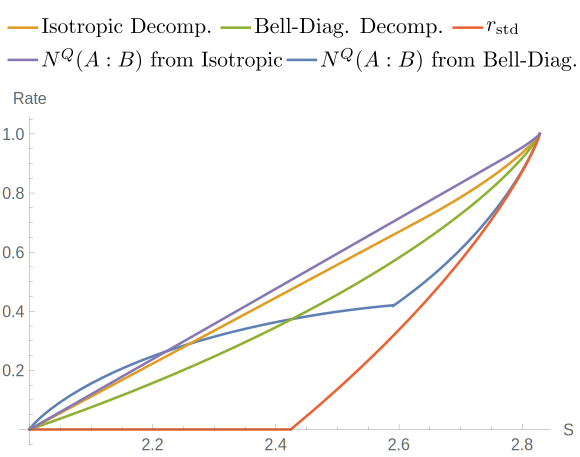
\includegraphics[height=0.7\textheight]{new_plot.pdf}
        \caption{Comparison of upper bounds for CHSH-based protocols}
      \end{figure}
  \end{onlyenv}
\end{frame}

\note{ Unfortunately, all of these are faithful. }

\begin{frame}{A Non-Faithful Upper Bound}
  \begin{itemize}[<+->]
    \item Werner states
      \[ \rho^{W,v} = v{\ket{\Psi_-}\bra{\Psi_-}} + \frac{1-v}{4}I \]
    \item No nonlocality for \(v < v_L \approx 0.6829\), nonlocality known for \(v \geq v_{NL} \approx 0.6964\)
    \item \(I(A:B \downarrow E) = 0\) for \(v < v_{\crit} \approx 0.7263 > v_{NL}\) via \emph{convex combination attack}, which requires measurement settings to be broadcast
  \end{itemize}

  \begin{onlyenv}<+->
    \begin{block}{Possible Approach}
      Can we prove the security of a non-broadcast protocol against quantum adversaries?
    \end{block}
  \end{onlyenv}
\end{frame}

\begin{frame}{A Convex Hull of Bounds}
  \begin{itemize}[<+->]
    \item \emph{Classical-classical (cc) squashed entanglement} \(E^{cc}_{sq,dev}(\rho, \sM, p(x,y))\)
      \[ \inf_{\substack{\sigma, \sN : \cP(\sigma, \sN) = \cP(\rho, \sM)}} \sum_{xy} p(x,y) \inf_{\cE_{x,y}} I{(A : B|E)}_{\cE_{x,y}(\psi^{\sigma})} \]
    \item Convex lower bound for convex combination attack and Bell-diagonal intrinsic information
    \item Upper bound for protocols with broadcast settings, Werner states, and only one basis
  \end{itemize}

  \begin{block}{Possible Approach}<+->
      What bounds on general protocols can we achieve using the cc-squashed entanglement?
  \end{block}
\end{frame}

\begin{frame}{Evaluation}
  \begin{itemize}[<+->]
    \item Most of these bounds are very difficult to compute
    \item If all optimisations are infima, any fixed choice provides an upper bound
    \item Many bounds are restricted to certain settings
  \end{itemize}

  \begin{block}{Possible Approach}<+->
      Are there any choices of states/measurements that will give greater insights? Can we simplify the optimisations? Can the restricted-setting bounds be generalised?
  \end{block}
\end{frame}

\subsection{Lower Bounds}

\begin{frame}{Asymmetric CHSH}
  \begin{itemize}[<+->]
    \item Asymmetric CHSH function
      \[ S_{\alpha} \coloneqq \alpha\angleb{A_0 B_0} + \alpha\angleb{A_1 B_0} + \angleb{A_0 B_1} - \angleb{A_1 B_1} \]
    \item Able to incorporate noisy preprocesing with probability \(q\)
    \item Requires three separate optimisations over different parameter regimes
    \item Minor improvement to key rate, but proof covers useful techniques that might be generalisable
  \end{itemize}
\end{frame}

\begin{frame}{Quasi-Relative Entropy}
  \begin{onlyenv}<1-3>
  \begin{itemize}[<+->]
    \item Main idea: bound the conditional entropy directly
    \item Express conditional entropy in terms of relative entropy
      \[ H{(A|E)}_{\rho} = -D(\rho_{AE}||I_A \otimes \rho_{E}) \]
    \item Use integral representation of logarithm
      \[ \ln\left(\frac{x}{y}\right) = \int_{0}^{1} \frac{x-y}{t(x-y) + y} \dif{t} \]
      in spectral integral representation of relative entropy
      \[ D(\rho||\sigma) = -\frac{1}{\ln 2} \int_{\R^{2}_{+}} \underbrace{\int_{0}^{1} \frac{y(x-y)}{t(x-y)+y} \dif{t}}_{y\ln(x/y)} \dif{\nu_{\rho,\sigma}(x,y)} \]
  \end{itemize}
  \end{onlyenv}

  \begin{onlyenv}<4->
  \begin{itemize}[<+->]
    \item Discretise integral representation of logarithm using \emph{Gauss-Radau quadrature} and commute the discrete sum with the spectral integral
      \[ D(\rho||\sigma) \leq \sum_{i=1}^m -\frac{w_i}{\ln 2} \underbrace{\int_{\R^{2}_{+}} \frac{y(x-y)}{t_i(x-y)+y} \dif{\nu_{\rho,\sigma}(x,y)}}_{D_{F_{t_i}}} \]
    \item Spectral integral of integral representation has a nice variational representation
      \[ D_{F_{t_i}} = \frac{1}{t}  \inf_Z \Tr\left[ \rho + \rho(Z + Z^{\dagger}) + (1-t)\rho{}Z^{\dagger}Z + t\sigma{}ZZ^{\dagger} \right]\]
  \end{itemize}
  \end{onlyenv}
\end{frame}

\note{
  If the phrase ``spectral integral'' scares you, just pretend that it's a normal evaluation of the expectation value of a function of two states, with \(x\) and \(y\) ranging over the eigenvalues, except it works for infinite-dimensional systems.
}

\begin{frame}{Calculating Conditional Entropy}
  \begin{itemize}[<+->]
    \item Need conditional entropy of classical Bell test data
    \item Must introduce Alice's measurement operators \(M_{a|x}\)
    \item Can impose additional constraints with Bob's measurement operators \(N_{b|y}\)
    \item Lower bound is always valid and converges for \(m\to\infty\)
    \item However, not possible to optimise efficiently
  \end{itemize}
\end{frame}

\begin{frame}{The NPA Hierarchy}
  \begin{itemize}[<+->]
    \item Assume states are pure, and replace operator Hilbert space requirement with commutation requirement
    \item Each sequence \(F\) of \(M_{a|x}\)'s and \(N_{b|y}\)'s is a \emph{monomial}, and \(F\ket{\psi}\) is a vector in the Hilbert space
    \item Higher levels of hierarchy \(\Rightarrow\) more monomials
    \item \emph{Gram matrix} with entries \(\braket{\psi|F_1^{\dagger}F_2|\psi}\) is \emph{positive semidefinite}
    \item Such matrices \alert{can be efficiently optimised over!}
    \item Some entries constrained by known statistics: \(\braket{\psi|M_{a|x}N_{b|y}|\psi} = p(ab|xy)\)
  \end{itemize}
\end{frame}

\begin{frame}{Evaluation}
  \begin{itemize}[<+->]
    \item QRE method is general, powerful, and reasonably fast
    \item Could possibly be adapted to compute upper bounds more efficiently
    \item These are just \emph{tools}: search space is unbelievably vast
    \item Closer analysis required to find structures
  \end{itemize}
  \begin{block}{Possible Approach}<+->
    Can quasi-relative entropies be used to compute upper bounds? What general conclusions can we draw about DIQKD key rates from these bounds?
  \end{block}
\end{frame}

\subsection{Nonlocality Monotones}

\begin{frame}{Monotones}
  \begin{itemize}[<+->]
    \item Functions of resources that \emph{preserve the pre-order} of the resources
      \[ R_1 \leadsto R_2 \Rightarrow \mu(R_1) \succeq \mu(R_2) \]
    \item Establish fundamental limits on achievable behaviours
      \[ \sWB(p) \subseteq \{ p' : \mu(p) \succeq \mu(p') \} \]
    \item Provide insight into structure of behaviour and wiring spaces
    \item Monotones known for multi-copy LO, but not multi-copy LOSR
  \end{itemize}
\end{frame}

\begin{frame}{Maximal Correlation}
  \begin{itemize}[<+->]
    \item Maximal correlation of two classical rvs \(A\) and \(B\)
      \[ \rho(A,B) = \max_{f,g} \frac{\E[(f(A)-\E[f(A)])(g(B)-\E[g(B)])]}{\sqrt{\Var[f(A)]\Var[g(B)]}} \]
      \begin{Array*}{rcl}
        \rho(A,B) = & \max_{f,g}  & \E[f(A)g(B)] \\
                    & \text{s.t.} & \E[f(A)] = \E[g(B)] = 0 \\
                    &             & \E[f(A)^2] = \E[g(B)^2] = 1,
      \end{Array*}
    \item Extend to conditional distributions: \(\rho(A,B|X,Y) = \max_{x,y} \rho(A,B|X=x,Y=y)\)
    \item \emph{Tensorisation}: multiple i.i.d.\ copies do not increase \(\rho\) \(\Rightarrow\) \(\rho\) is a monotone with \(\succeq = \geq\)
  \end{itemize}
\end{frame}

\begin{frame}{Related Measures}
  \begin{itemize}[<+->]
    \item Hypercontractivity (HC) and maximal correlation (MC) ribbons are subsets of \({[0,1]}^2\)
    \item Ribbons expand under wiring:
      \[ \HC(A,B) \subseteq \HC(A',B'), \MC(A,B) \subseteq \MC(A',B') \]
    \item Ribbons are monotones with \(\succeq = \subseteq\)
    \item Properties of \(\rho\) derived from ribbons
    \item \(\rho\) can be efficiently computed, ribbons cannot!
  \end{itemize}
\end{frame}

\begin{frame}{Maximal Correlation Over Behaviours}
\end{frame}

\begin{frame}{Desiderata}
  \begin{enumerate}[<+->]
    \item Easy to compute \(\mu(p)\)
    \item \(\{ p : \mu(p) = \mu' \}\) can be efficiently optimised over
    \item Tight: if \(\mu(p) = \mu(p')\), there exists a wiring \(p \mapsto p'\)
    \item If \(\mu(p) = \mu(p')\), wiring for \(p \mapsto p'\) can be expicitly constructed
  \end{enumerate}
\end{frame}

\begin{frame}{Evaluation}
  \begin{itemize}[<+->]
    \item \(\rho\) is easy to compute but probably not tight
    \item Effect of shared randomness unclear
    \item Potentially rich area to explore
    \item Caveat: we want something like
      \[ \max_{E|AB} \frac{H(A|E) - H(A|B)}{H(A)} \leq f(\rho(A,B)) \]
  \end{itemize}
\end{frame}

\section*{Conclusion}

\begin{frame}[c]{}
  \begin{center}
    \begin{beamercolorbox}[sep=8pt,center,shadow=true,rounded=true]{title}
      Thank you!
    \end{beamercolorbox}
  \end{center}
\end{frame}

% Placing a * after \section means it will not show in the
% outline or table of contents.

\end{document}

